%%% Event Triggers
%%%
%%% PostgreSQL already did have Triggers, targeting Data Modification. Now
%%% in 9.3 it's proposing Triggers on Events. What events? What do you mean?
%%% What can such a trigger do, based on what information?
%%%
%%% All you ever wanted to know about that new PostgreSQL feature, how it
%%% works and how to use it.

\documentclass{beamer}

\usepackage{minted}
%% \usemintedstyle{emacs}
\usepackage{beamerthemesplit}
\usepackage[utf8]{inputenc}
%% \usetheme{AnnArbor}
\usetheme{Boadilla}
%% \usetheme{Pittsburgh}
%% \usecolortheme{beaver}
\beamertemplatetransparentcovered

\title{Event Triggers}
\subtitle{A.K.A The Real Mess.}
\author{Dimitri Fontaine \texttt{dimitri@2ndQuadrant.fr}}
\date{February, 3rd 2013}
\logo{
\includegraphics[height=0.4cm]{2ndQuadrant-cross.png}}

\begin{document}

\frame{\titlepage}

\section{Introduction}

\begin{frame}[fragile]
  \frametitle{Dimitri Fontaine}

  \begin{center}
    \textbf{2ndQuadrant France}
    \newline
    PostgreSQL Major Contributor
  \end{center}

  \vfill

\begin{columns}[c]
\column{.75\textwidth} 

  \begin{itemize}
   \item<2-> \texttt{pgloader}, \texttt{prefix}, \texttt{skytools}, \texttt{debian}, …
   \item<2-> \texttt{\textbf{CREATE EXTENSION}}
   \item<3-> \texttt{\textbf{CREATE EVENT TRIGGER}}
   \item<3-> \textit{Bi-Directional Réplication}
   \item<4-> \textit{Partitionning}
  \end{itemize}  

\column{.25\textwidth}
\begin{center}
  
\includegraphics[height=5em]{bulle-blue-icon.png}
\end{center}
\end{columns}
\end{frame}

\frame{
  \frametitle{Event Triggers}

  \begin{center}
    So, \textbf{Event Triggers}, what do you mean?
    \vfill

    \begin{center}
      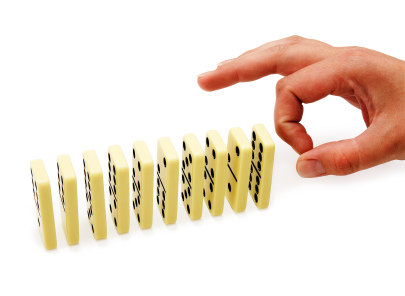
\includegraphics[height=2.1in]{event-trigger.jpg}
    \end{center}
  \end{center}
}

\begin{frame}[fragile]
  \frametitle{SQL primer \texttt{1/3}}

  \center{It always starts \textit{simple}}
  \vfill

\begin{minted}{postgresql}
create table foo(a text, b int);

select a, b
  from relation r
 where a > '2013'
\end{minted}
\end{frame}

\begin{frame}[fragile]
  \frametitle{SQL primer \texttt{2/3}}

  \center{It always starts \textit{simple enough}}
  \vfill

\begin{minted}{postgresql}
create table foo(a int, b int);

select a, b
  from relation r
 where a > '2013'
\end{minted}
\end{frame}

\begin{frame}[fragile]
  \frametitle{SQL primer \texttt{3/3}}

  \center{It always starts \textit{simple}... then we try handling \textit{time}}
  \vfill

\begin{minted}{postgresql}
create table foo(a date, b int);

select a, b
  from relation r
 where a > '2013'
\end{minted}
\end{frame}

\section{PostgreSQL Extensions}

\begin{frame}[fragile]
  \frametitle{SQL primer: Extensions}

\begin{minted}{postgresql}
create extension hstore;

create table testhstore (h hstore);

select count(*)
  from testhstore
 where h @> 'wait=>CC, public=>t';
\end{minted}
\end{frame}

\frame{
  \frametitle{PostgreSQL supports Extensions}

  \center{Data Type Specific Indexing and Query Support}
  \vfill

  \begin{itemize}
    \item Functions, Aggregates, Window Functions
    \item Data Types with Input/Output functions
    \item Casts (implicit, assignment only)
    \item Operators
    \item Operator Class, Operator Family
    \item \textit{and more...}
  \end{itemize}
}

\section{Data Modification Trigger}

\frame{
  \frametitle{Physical Model Optimisations, Business Logic}

  \center{With PostgreSQL you can tweak \texttt{INSERT}, \texttt{UPDATE}, \texttt{DELETE}}

  \vfill

  \begin{itemize}
    \item<1-> Maintain a Materialized View
    \item<1-> Apply crossing threshold discounts
    \item<2-> Trigger external actions on some events
    \item<2-> \texttt{NOTIFY} some other application parts (e.g. cache)
    \item<3-> Queue events to process later (Use \alert{PGQ})
    \item<3-> Replicate data (Slony, Londiste, Bucardo...)
  \end{itemize}
}

\begin{frame}[fragile]
  \frametitle{Data Modification Trigger Example \texttt{1/2}}

\begin{minted}{postgresql}
CREATE TABLE main_table (a int, b int);

CREATE FUNCTION trigger_func()
        RETURNS trigger
       LANGUAGE plpgsql AS '
BEGIN
  RAISE NOTICE ''trigger_func(%) called: action = %, when = %, level = %'',
               TG_ARGV[0], TG_OP, TG_WHEN, TG_LEVEL;
  RETURN NULL;
END;';
\end{minted}
\end{frame}

\begin{frame}[fragile]
  \frametitle{Data Modification Trigger Example \texttt{2/2}}

\begin{minted}{postgresql}
    CREATE TRIGGER before_ins_stmt_trig
  BEFORE INSERT ON main_table
          FOR EACH STATEMENT
 EXECUTE PROCEDURE trigger_func('before_ins_stmt');

    CREATE TRIGGER after_ins_stmt_trig
   AFTER INSERT ON main_table
          FOR EACH STATEMENT
 EXECUTE PROCEDURE trigger_func('after_ins_stmt');
\end{minted}
\end{frame}

\section{Event Triggers}

\begin{frame}[fragile]
  \frametitle{SQL \textbf{\texttt{DDL}} primer}

  \center{Data Definition Language}
  \vfill

\begin{minted}{postgresql}
create table foo
 (
   id serial primary key,
   f1 text
 );

 alter table foo
  add column f2 text check (upper(f2) = f2);
\end{minted}
\end{frame}

\begin{frame}[fragile]
  \frametitle{SQL \textbf{\texttt{DDL}} primer}

  \center{Here's what \texttt{foo} looks like now}
  \vfill

\begin{minted}{postgresql}
~# \d foo
                         Table "public.foo"
 Column |  Type   |                    Modifiers                     
--------+---------+--------------------------------------------------
 id     | integer | not null default nextval('foo_id_seq'::regclass)
 f1     | text    | 
 f2     | text    | 
Indexes:
    "foo_pkey" PRIMARY KEY, btree (id)
Check constraints:
    "foo_f2_check" CHECK (upper(f2) = f2)
\end{minted}
\end{frame}

\frame{
  \frametitle{What if you could \textit{tweak} \texttt{DDL} too}

  \center{Some \textbf{DDL} Trigger use cases}
  \vfill

  \begin{itemize}
  \item Audit trail
  \item Replication Triggers
  \item Implement Local Policies
  \item Divert Execution
  \item Limited Granting of DDL privileges with \texttt{Security Definer}
    trigger functions
  \end{itemize}
}

\frame{
  \frametitle{What if you could \textit{tweak} \texttt{DDL} too}

  \center{Some \textbf{Event} Trigger use cases}
  \vfill

  \begin{itemize}
  \item<1-> \texttt{sql\_drop} (\texttt{CASCADE})
  \item<2-> Prevent Table Rewrite (except at night) (unless full moon)
  \item<3-> Create Table If Not Exists, at \texttt{INSERT} time
  \item<4-> Integrated Extension Package Management
  \end{itemize}
}

\section{Using Event Trigger}

\begin{frame}[fragile]
  \frametitle{Event Trigger Primer}

\begin{minted}{postgresql}
CREATE OR REPLACE FUNCTION abort_any_command()
  RETURNS event_trigger
 LANGUAGE plpgsql
  AS '
BEGIN
  RAISE EXCEPTION ''command % is disabled'', tg_tag;
END;
';

CREATE EVENT TRIGGER abort_ddl ON ddl_command_start
   EXECUTE PROCEDURE abort_any_command();
\end{minted}
\end{frame}

\begin{frame}[fragile]
  \frametitle{Event Trigger Primer}

\begin{minted}{postgresql}
ALTER EVENT TRIGGER abort_ddl DISABLE;
DROP EVENT TRIGGER abort_ddl DISABLE;
\end{minted}
\end{frame}

\frame{
  \frametitle{Events}

  \center{Limited Number of Events Supported now}
  \vfill

  \begin{itemize}
    \item \texttt{ddl\_command\_start}
    \item \texttt{ddl\_command\_end}
    \item \texttt{sql\_drop} \textit{currently in review}
  \end{itemize}
}

\frame{
  \frametitle{Information}

  \center{}
  \vfill

  \begin{itemize}
    \item
    \item
    \item
  \end{itemize}
}

\section{Conclusion}

\frame{
  \frametitle{Conclusion}

  \begin{center}
    Any Question? Now is the time to ask!

    \vfill

    \begin{center}
      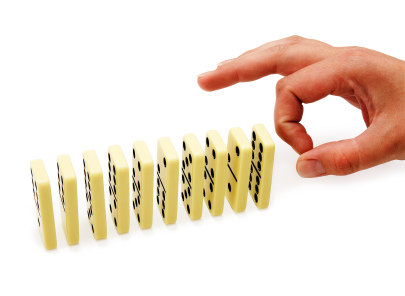
\includegraphics[height=2.1in]{event-trigger.jpg}
    \end{center}
  \end{center}
}

\end{document}
